

\frame{

\tableofcontents[sectionstyle=show/hide,hideothersubsections]

}


\subsection{Présentation, objectifs} % communauté

\frame{
\frametitle{UIMA: Introduction}
\begin{itemize}
\item Unstructured Information Management Applications:
\begin{itemize}
\item {\bf Spécification} définie par l'OASIS {\small (Organization for the Advancement of Structured Information Standards)}
\item {\bf Implémentation} initiée par IBM, reprise par Apache (2006)
\end{itemize}

\item But : encourager l'{\bf interopérabilité entre composants}
\begin{itemize}
\item {\em Représentation des données,} indépendance artefact / méta-données
\item {\em Modélisation/échanges de données} indépendants de la plateforme, forme ``programmable''
\item {\em Découverte, ré-utilisation et composition} de composants indépendants
\item {\em Interopérabilité au niveau services}
\end{itemize}
\end{itemize}
}

\frame{
\frametitle{Apache UIMA}

\begin{itemize}
\item Une implémentation {\bf Java} de la spécification UIMA OASIS
\item Un {\em framework} + un {\em SDK}:
\begin{itemize}
\item SDK : ensemble d'outils pour construire des composants UIMA via API
\item framework : librairies suffisantes pour déployer des composants
\end{itemize}
\item Open-source
\item Un projet Apache dynamique:
\begin{itemize}
\item Version 2.3 $\approx$ Janvier 2010, prochaine version bientôt
\item Apache ``top-level project'' depuis Mai 2010
\item Communauté d'utilisateurs grandissante (?)
\item Liste(s) d'utilisateurs active(s)
\end{itemize}
\end{itemize}

}

\subsection{Concepts généraux}

\frame{
\frametitle{Principe}
\begin{itemize}
\item Chaîne de traitement composée de:
\begin{itemize}
\item un {\em Collection Reader}, qui lit le(s) document(s)
\item une séquence d'{\em Annotator Engine (AE)}, procédant chacun à une tâche donnée
\item un/plusieurs AEs qui ``consomment'' le résultat {\footnotesize (ex- {\em CAS Consumers})}
\end{itemize}
\item Le CAS {\em (Common Analysis Structure)} contient :
\begin{itemize}
\item le document de départ (String)
\item les annotations (méta-données) ajoutées par les composants
\item le {\em Type System} 
\begin{itemize}
\item typologie pour la représentation des méta-données
\end{itemize}
\end{itemize}
\item Gestion du processus par le framework via un {\em Collection Processing Engine (CPE)} 
\begin{itemize}
\item Passage de paramètres, gestion d'erreurs, ``flot'' (e.g. parallélisation), ressources, log...
\end{itemize}
\end{itemize}
}

\frame{
\noindent\begin{center}
\noindent\hspace*{-.7cm}\scalebox{.35}[.4]{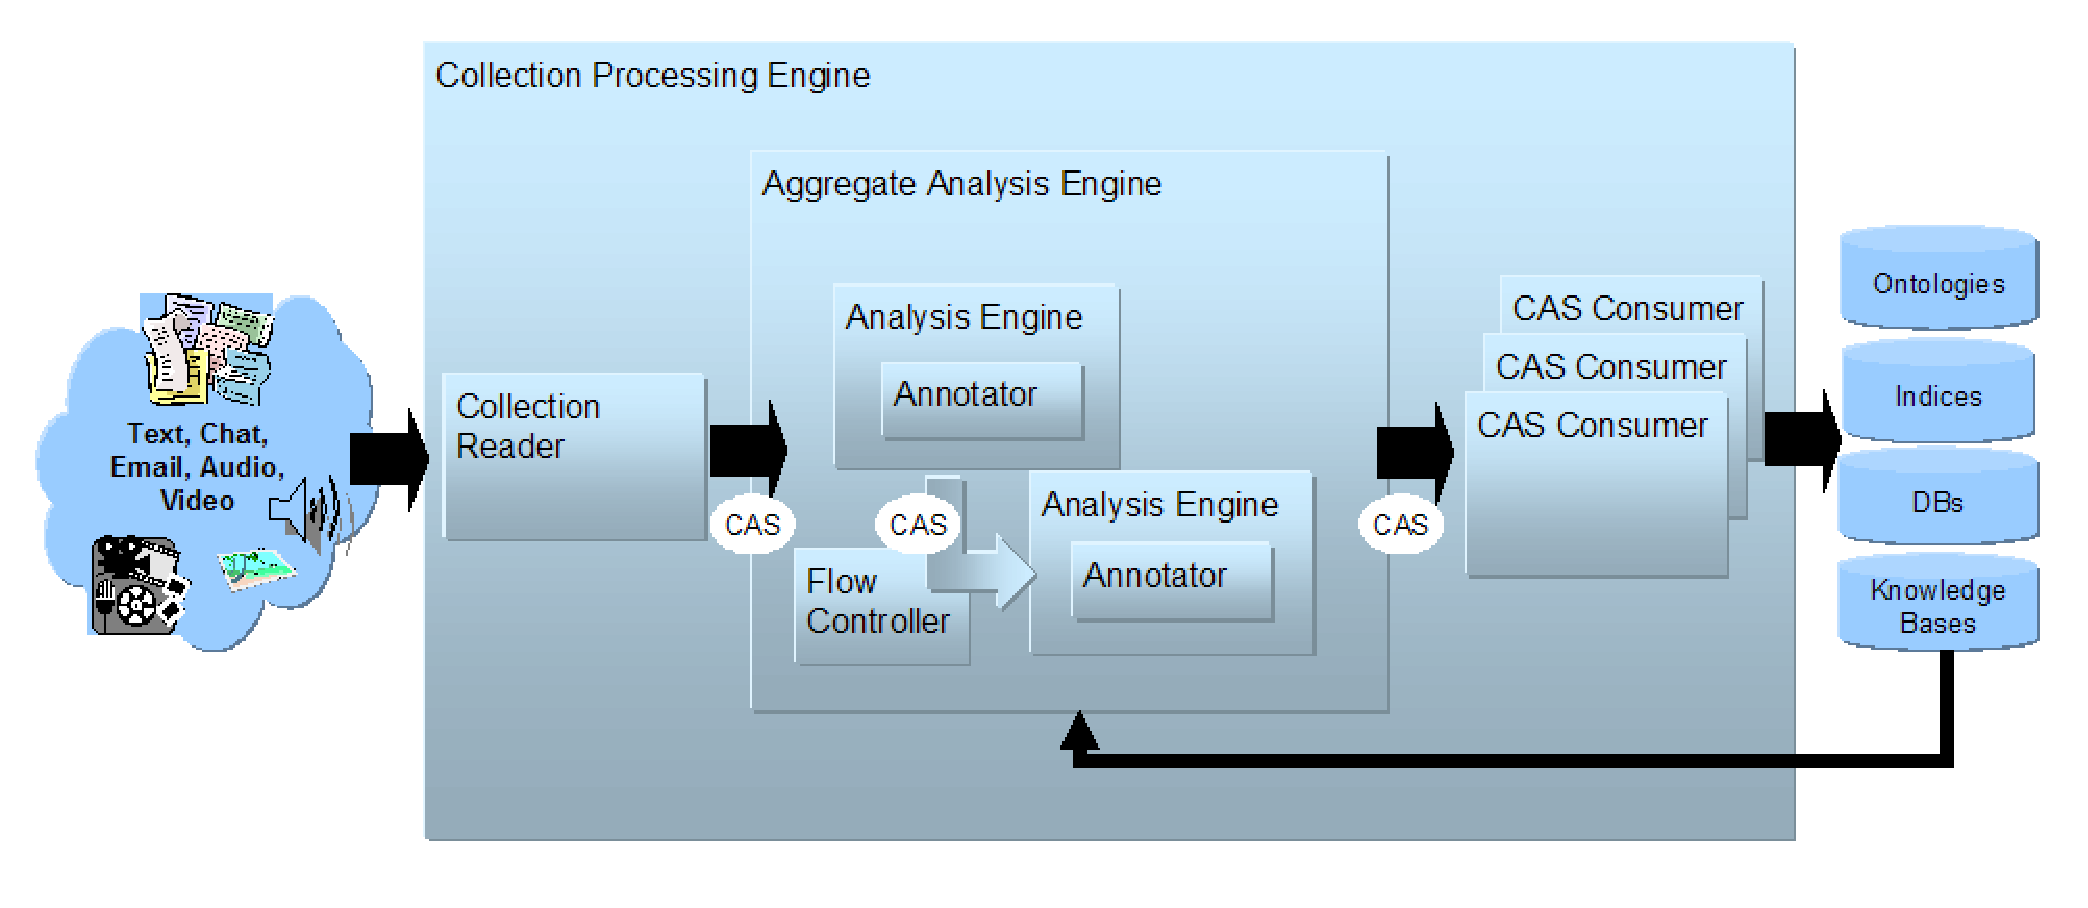
\includegraphics{uima_process.eps}}
\end{center}

}


\subsection{Type System}

\frame{
\frametitle{Représentation des méta-données: le Type System}

\begin{itemize}
\item Hiérarchie de types destinés à ``recevoir'' les annotations
\item un type peut comporter des attributs {\em (features)}
\begin{itemize}
\item ex: {\tt Individu} avec features {\tt nom}, {\tt prenom} de type {\tt String}
\item typage des features parmi types primitifs UIMA + tout type précédemment défini
\end{itemize}
\item Héritage classique
\begin{itemize}
\item ex: {\tt Chercheur} hérite de {\tt Individu}, feature {\tt h\_index} ajoutée.
\end{itemize}
\item Annotation (instance d'un type) accédée via objet Java 
\item[$\rightarrow$] {\bf MAIS} Type UIMA $\neq$ objet Java
\begin{itemize}
\item aucune méthode spécifique associée (accesseurs seuls)
\item interfaces/classes abstraites impossibles
\end{itemize}
\item Type standard {\tt org.apache.uima.jcas.tcas.Annotation}
\begin{itemize}
\item Features {begin}/{end} de type {int} = position dans le texte
\end{itemize}
\end{itemize}
}

\subsection{Annotateurs}

\frame{
\frametitle{Construire un annotateur}
\begin{itemize}
\item {\em Annotator Engine Descriptor} (fichier XML):
\begin{itemize}
\item Nom de la classe Java
\item Type System
\item Paramètres spécifiques
\begin{itemize}
\item Nommage, typage, description, affectation
\item NB: entrée/sortie = CAS
\end{itemize}
\item {\em Capabilities}: types nécessaire en entrée et fournis en sortie
\end{itemize}
\item Classe Java héritant de {\tt JCasAnnotator\_ImplBase}
\begin{itemize}
\item Méthode {\tt initialize(context)} : gestion des paramètres
\item Méthode {\tt process(aJCas)} : tâche proprement dite
\begin{itemize}
\item Accès au document : {\tt aJCas.getDocumentText()}
\item Accès aux annotations avec itérateurs : {\tt aJCas.getAnnotationIndex(myType).iterator()}
\item Écriture d'annotations : {\tt myAnnot = new MyType(aJCas)} ... {\tt myAnnot.addToIndexes()}
\end{itemize}
\end{itemize}
\end{itemize}
}

%\frame{
%\frametitle{Autres composants (aperçu)}

%\begin{itemize}
%\item {\em Collection Reader
%\end{itemize}
%}

\subsection{Outils standard UIMA}
\frame{
\frametitle{Outils (aperçu)}
\begin{itemize}
\item API pour gestion d'erreurs, {\em logging}, etc. 
\item Composant {\em Collection Reader} qui lit les fichiers $\rightarrow$ CAS
\item Composant {\em CAS consumer} qui écrit les données annotées en XML (format XMI)
\item Outils graphiques
\begin{itemize}
\item Costruction de descripteurs TS, AED (Eclipse)
\item Composition/configuration de CPE
\item Visualisation d'annotations
\end{itemize}
\item Nombreuses façons d'utiliser/lancer un traitement :
\begin{itemize}
\item CPE GUI (graphique)
\item script UIMA
\item programme Java
\end{itemize}
\end{itemize}
}


\subsection{Synthèse}


\frame{
\frametitle{Le framework UIMA : synthèse}

\begin{itemize}
\item Objectif essentiel : favoriser la {\bf compositionnalité} entre composants d'analyse
\item Moyen : {\bf standardisation} 
\begin{itemize}
\item de la représentation des données 
\item de ``l'interfaçage'' des composants (E/S, paramètres, etc.)
\end{itemize}
\item Difficultés :
\begin{itemize}
\item éviter de restreindre l'éventail des tâches représentables
\item rester $\approx$ simple à utiliser (développeur/utilisateur)
\item efficacité
\end{itemize}
\item Bénéfices secondaires :
\begin{itemize}
\item Librarie d'outils standard
\item Accès aux composants extérieurs existants
\end{itemize}
\end{itemize}
}

\frame{
\frametitle{Adopter UIMA ? (avis subjectif)}
\begin{itemize}
\item Inconvénients :
\begin{itemize}
\item Contraignant $\rightarrow$ construction + complexe, utilisation + laborieuse
\item Chronophage $\rightarrow$ apprentissage/adaptation, + de cas à gérer, - de marge de man\oe uvre
\item Rentabilité ? $\rightarrow$ moyen/long terme 
\begin{itemize}
\item Quand une ``masse critique'' de composants est disponible
\item Si ce standard reste dynamique
\end{itemize}
\end{itemize}
\item Avantages :
\begin{itemize}
\item Standardisation : modularité, flexibilité, communication
\item Favorise programmation ``propre'' 
\begin{itemize}
\item sinon, UIMA inutile !
\end{itemize}
\item[$\Rightarrow$] Bénéfice UIMA $\approx$ langage non structuré vs. structuré
\begin{itemize}
\item contraignant d'abord, rentable ensuite
\item + robuste, débuggage simplifié, maintenance facilité...
\end{itemize}
\end{itemize}
\end{itemize}
}


% pbms fréquents chemins, pratique nécessaire, apprentissage
